\documentclass[titlepage]{article}

% Package Information
\usepackage[margin=1in]{geometry}
\usepackage[hidelinks]{hyperref}
\usepackage{graphicx}
\usepackage{float}

% Title Information
\title{Overview of the Electrical Team}
\author{University of Calgary Solar Car Team\\
        Electrical Technical Documentation Team}
\date{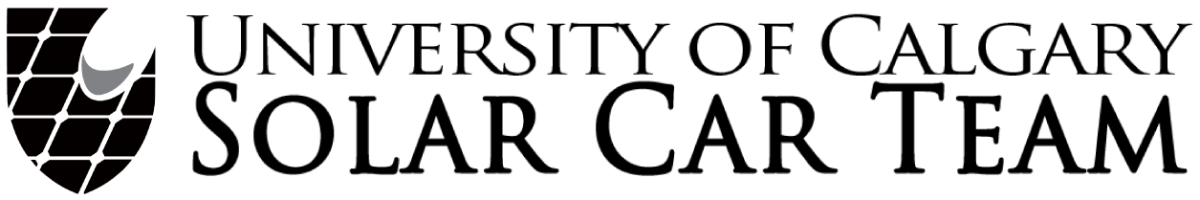
\includegraphics{images/logo.png}}

\begin{document}
    \maketitle

    \section{Introduction}
    The electrical team deals with all of the electrical work for the
    University of Calgary Solar Car project. The electrical work can be
    broken down into roughly four basic areas of work; the four areas
    roughly are PCB design, the electrical systems, the battery system,
    and the solar arrays. 
    \section{PCB Design}
    The PCB work for the car is done by our PCB design team. All of our
    PCBs are designed in Altium PCB designer. A list of the PCBs 
    designed for the solar car is given below
    \begin{itemize}
        \item The AUX BMS
        \item The DC-DC Converter
        \item The CCS
        \item The Lights Board
        \item The Driver Control Board
        \item The CAN Spliter
        \item The Fan Board
        \item The Audio Board
        \item The Strobe Board
        \item The Relay Board
    \end{itemize}
    Some of the more complex boards will be discussed bellow
    \subsection{The Central Control System}
    The Central Control System or CCS is a board designed to control the
    CAN network of the car. The primary use of the CCS in the car is 
    sending data from the CAN network to the Raspberry Pis. A picture of
    the CCS hardware is given in figure \ref{fig:css}
    \begin{figure}[H]
        \centering
        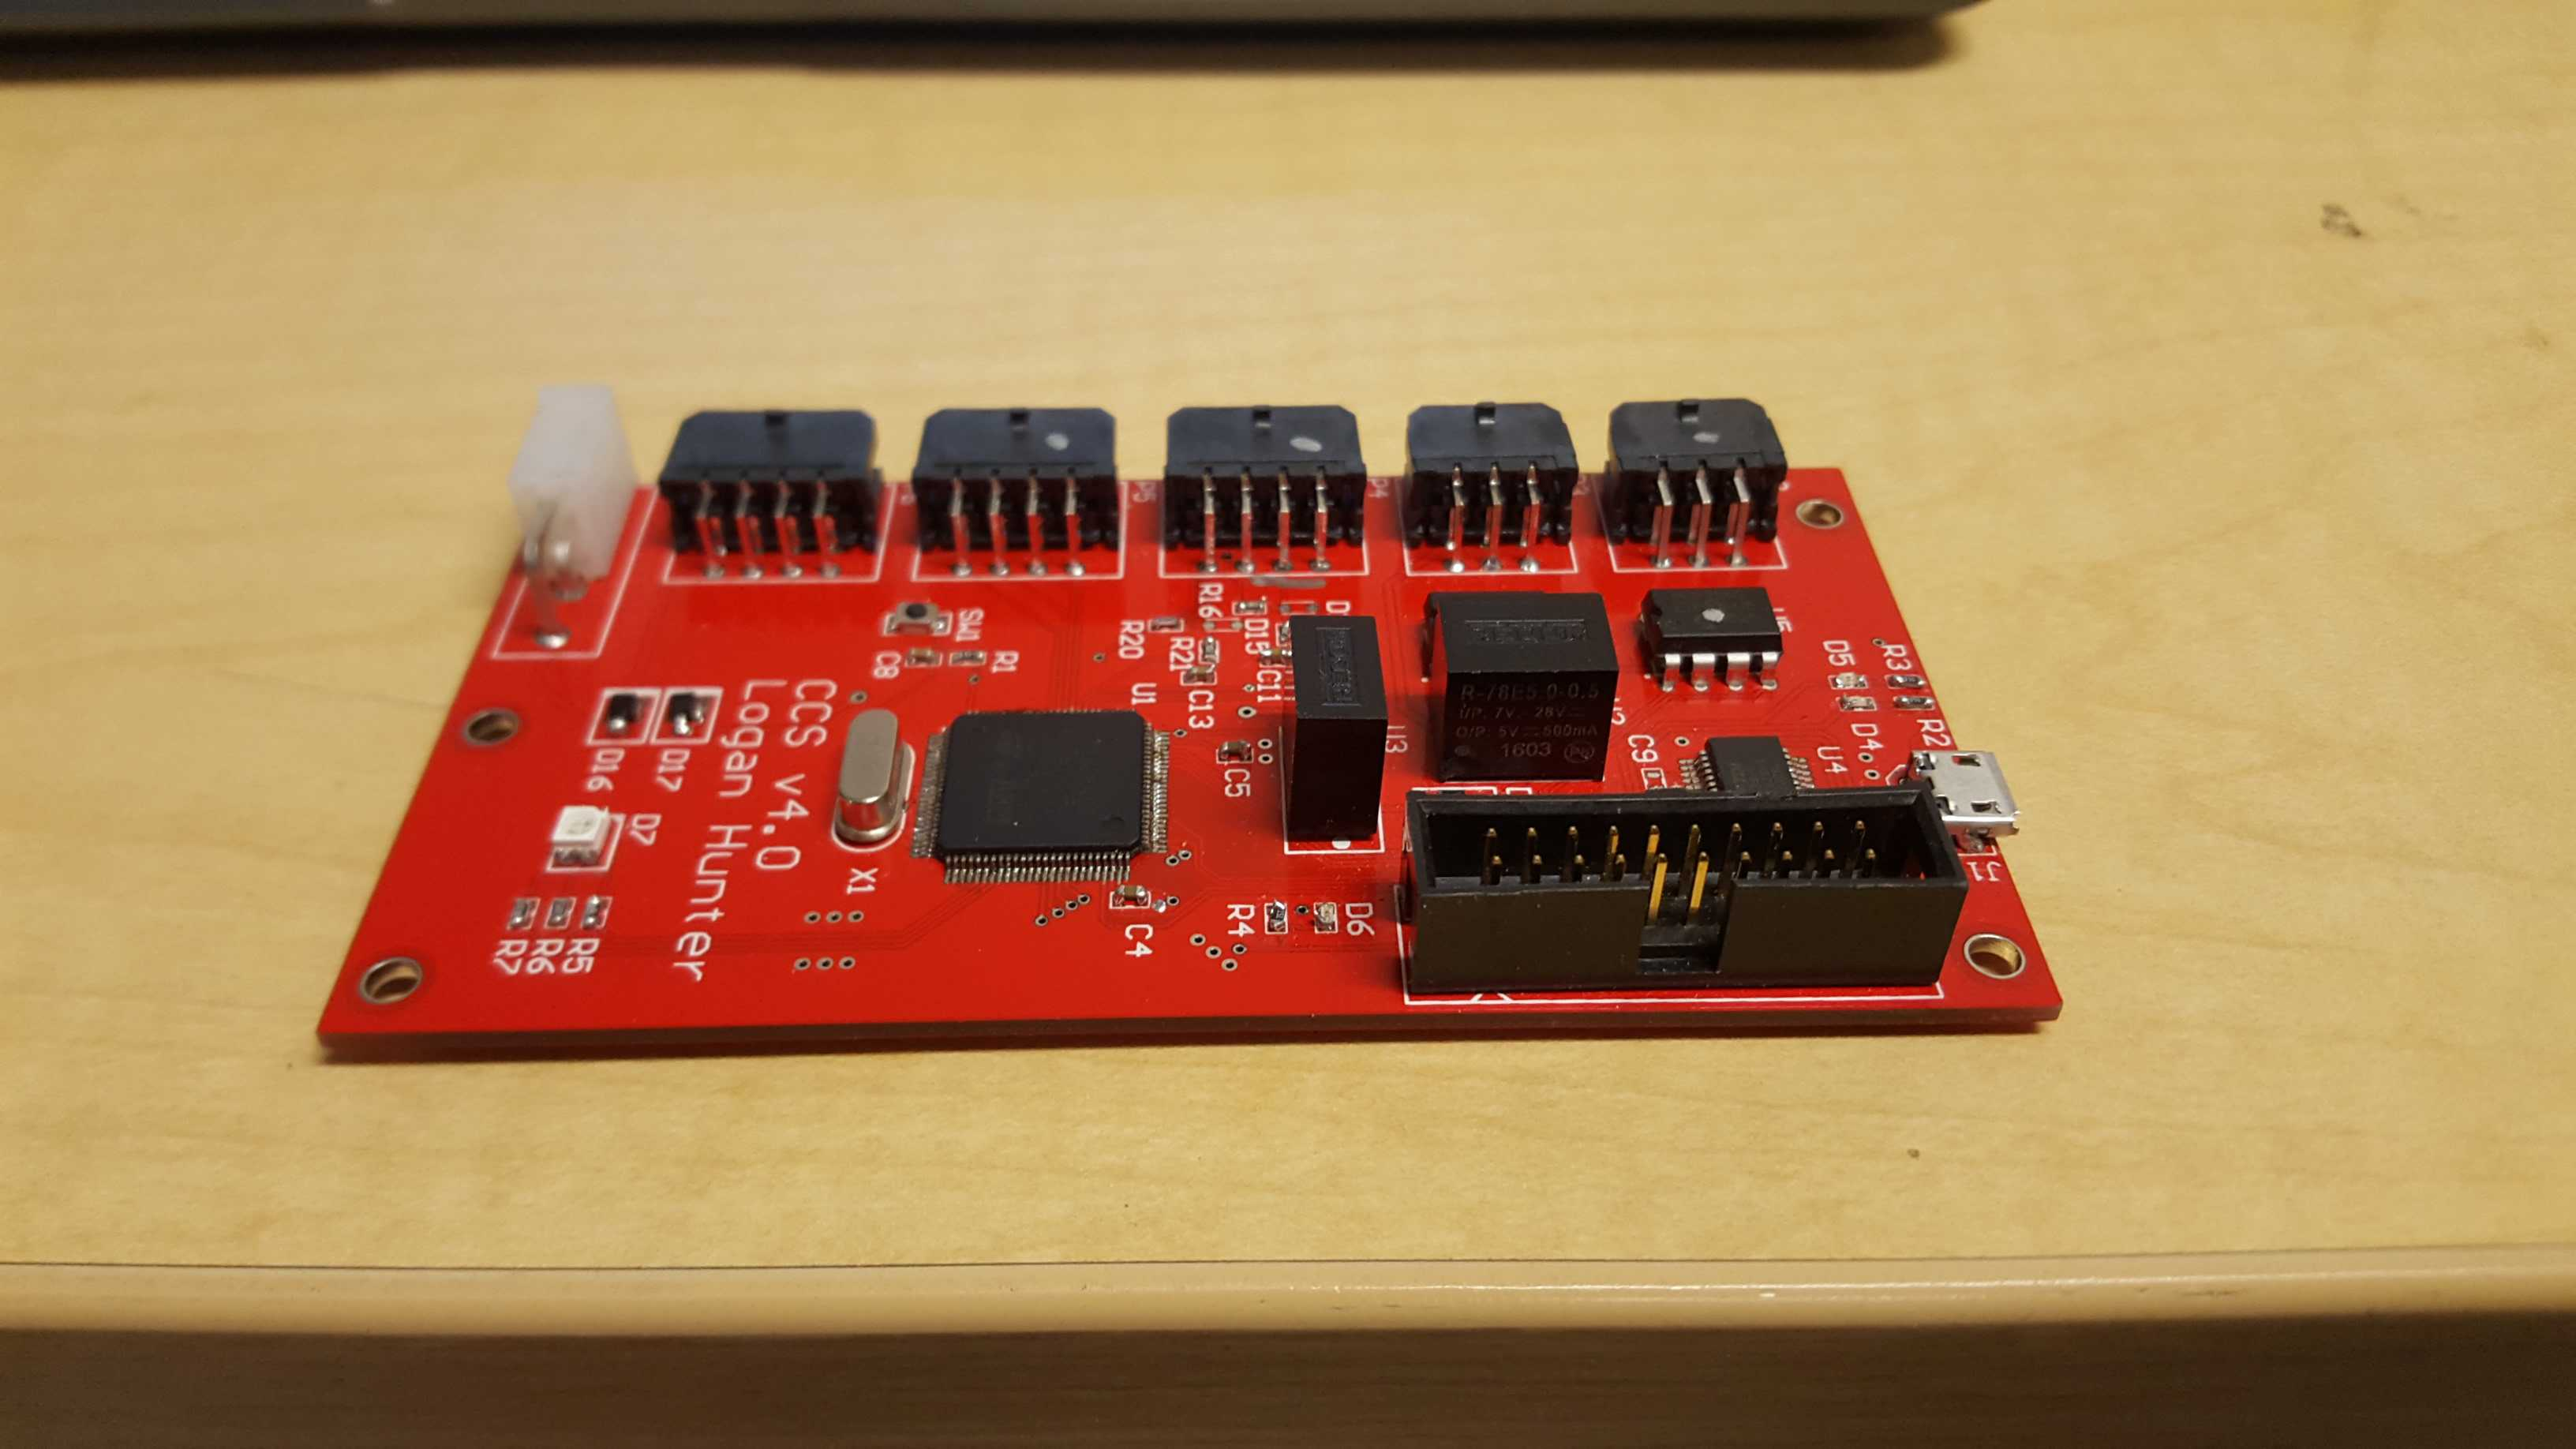
\includegraphics[width=0.5\textwidth]{images/ccs.jpg}
        \caption{The CCS board Hardware}
        \label{fig:css}
    \end{figure}
    \subsection{The Driver Control Board}
    The driver control board manages all driver inputs from the car and
    distributes the inputs over the CAN network. The inputs include but
    are not limited to acceleration and regen brake pedals, buttons for
    lights, drive control. A picture of the driver control hardware is
    given in figure \ref{fig:driver}
    \begin{figure}[H]
        \centering
        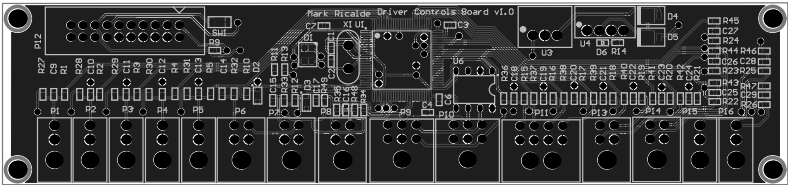
\includegraphics[width=0.5\textwidth]{images/driver.png}
        \caption{The Driver Control Hardware Schematic, as designed in
                 Altium}
        \label{fig:driver}
    \end{figure}
    \subsection{The Lights Board}
    The purpose of the lights board is to control all of the lights on
    the car, such as the headlights. The basic operation of the lights
    board the CAN network will tell the lights board which lights to
    turn on and then the board will send power to the necessary lights.
    Future upgrades that the team would want to make to the light board
    include integration of the emergency strobe board into the lights
    board and a sufficient power system to run the cars horn on. A
    picture of the lights board is given in figure \ref{fig:lights_HW}.
    \begin{figure}[H]
        \centering
        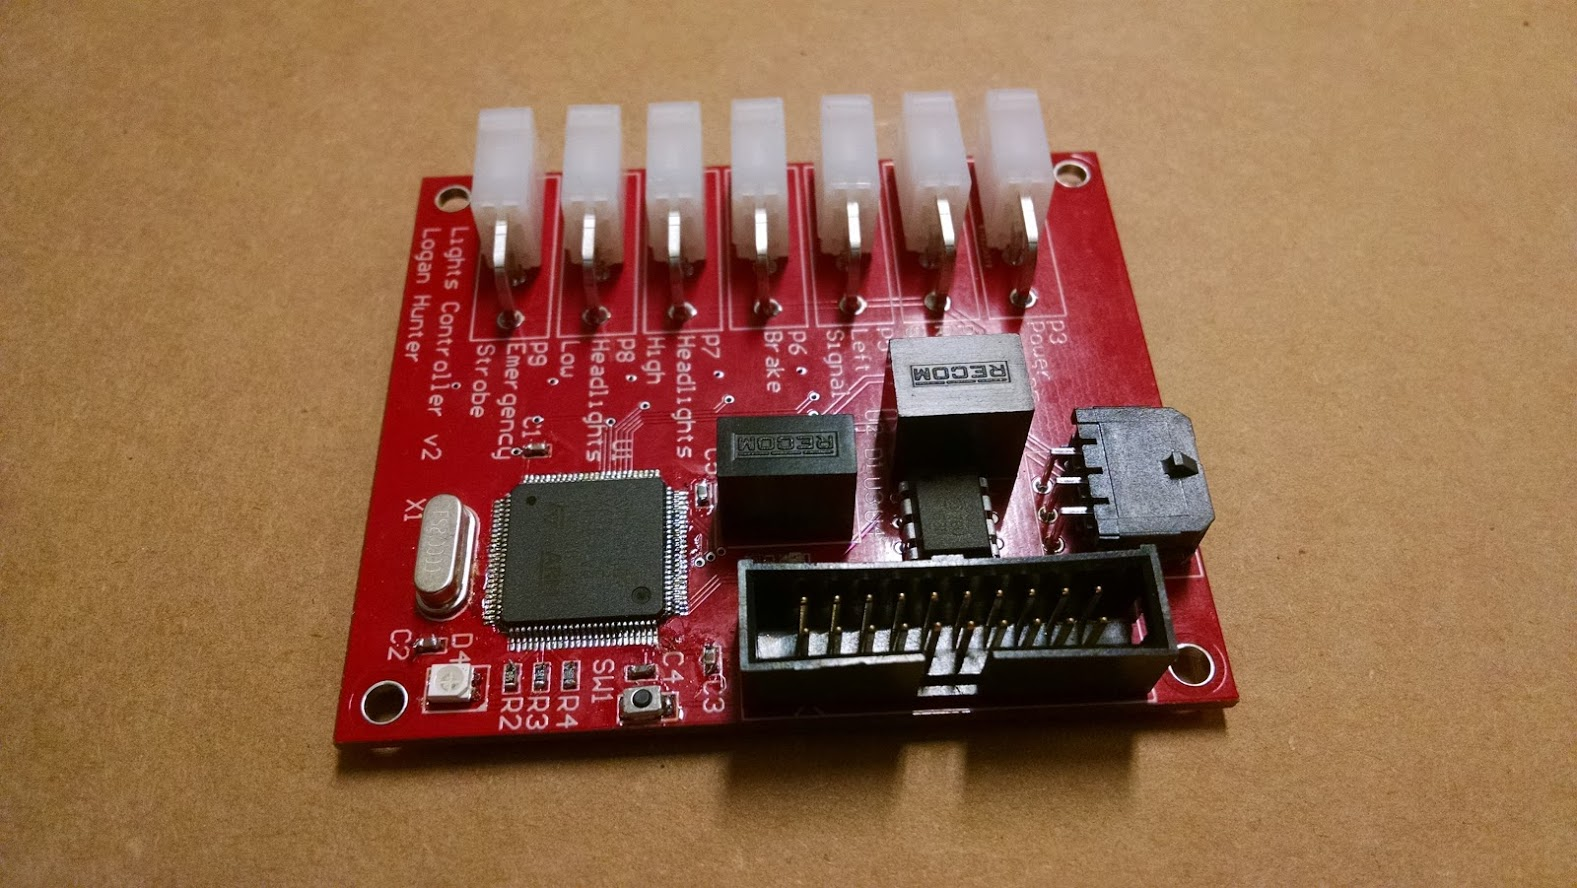
\includegraphics[width=0.5\textwidth]{images/light_board.jpeg}
        \caption{The Lights Board Hardware}
        \label{fig:lights_HW}
    \end{figure}
    \subsection{The Audio Board}
    The audio board will be used to add a media player into the solar
    car. It is designed to take aux input from a phone or other audio
    source and send it to two speakers which will be integrated into the
    car. The audio board is currently under active development. A
    picture of the audio board hardware is given in figure
    \ref{fig:audio}
    \begin{figure}[H]
        \centering
        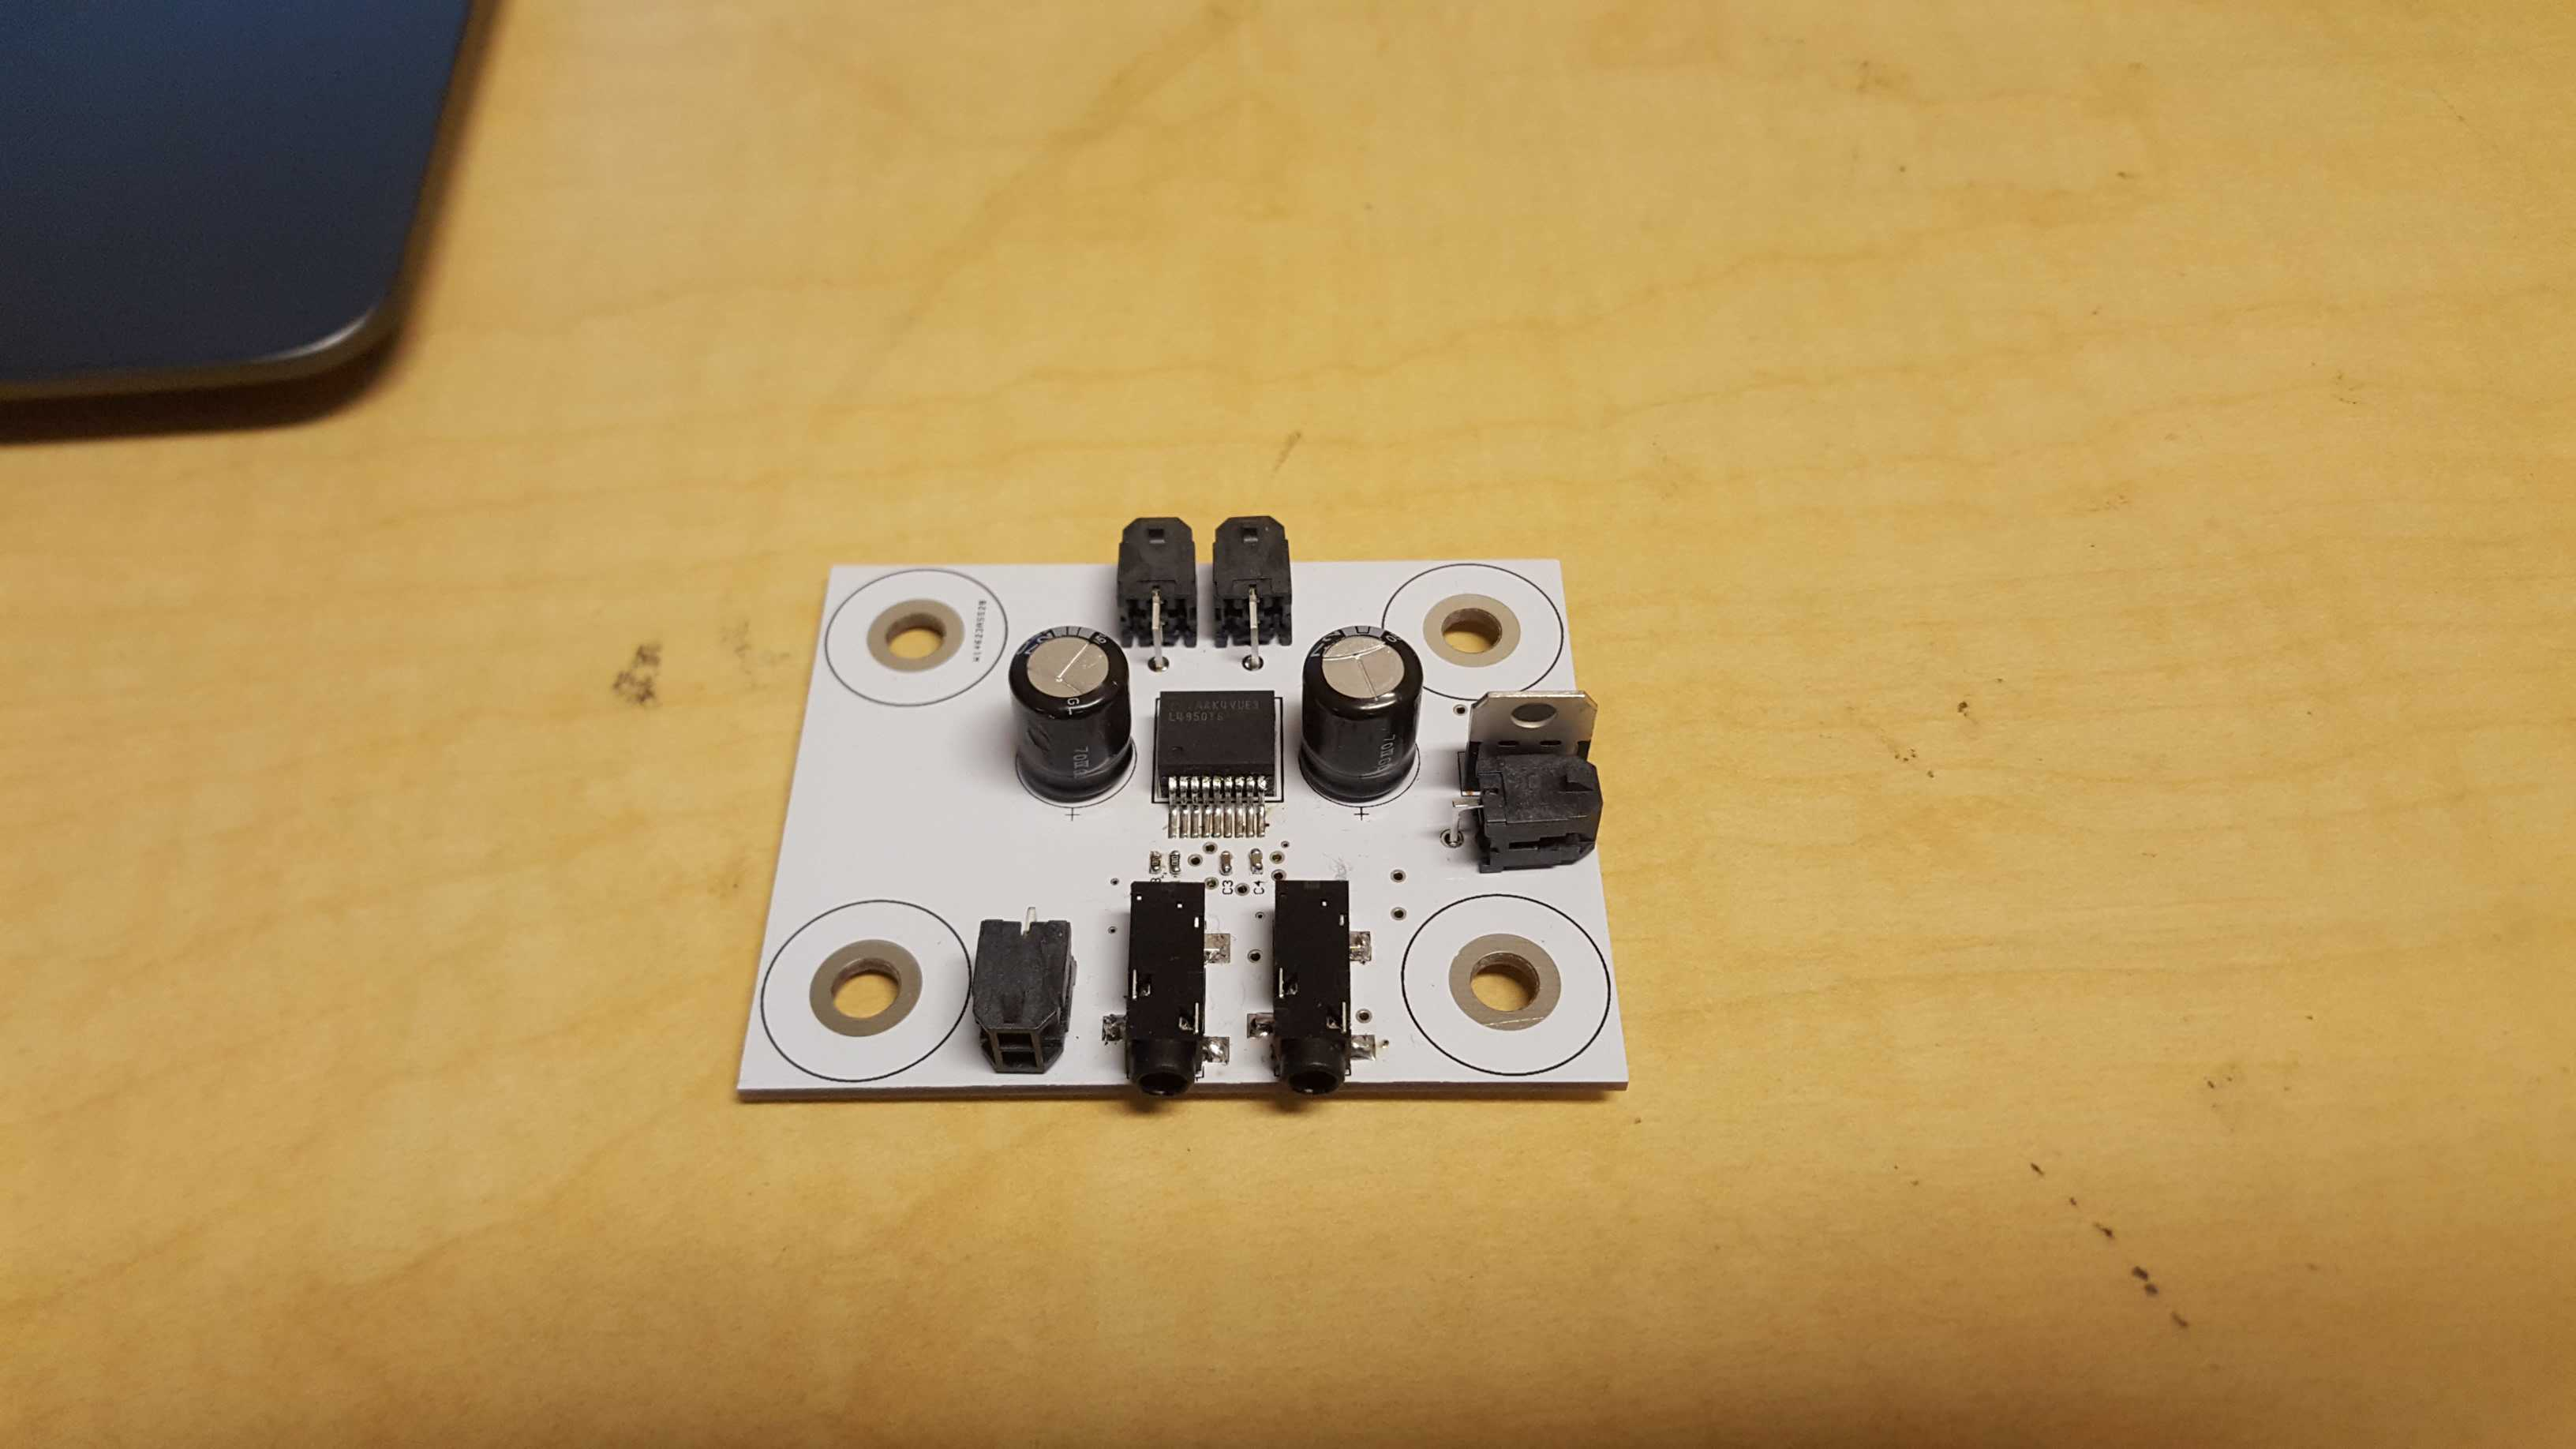
\includegraphics[width=0.5\textwidth]{images/audio_board.jpg}
        \caption{The Audio Board Hardware}
        \label{fig:audio}
    \end{figure}
    The AUX BMS and DC-DC converter will be talked about with the
    battery as they are directly inside the battery.
    \section{Electrical Systems}
    \section{Battery Systems}
    \section{Solar Arrays}
\end{document}
